% \%setchapterpreamble[u]{\margintoc}
%\chapter{Einleitung}
%\labch{intro}


% \setchapterimage[6cm]{donut.jpg}
\setchapterpreamble[u]{\margintoc}
\chapter{Einleitung}
\labch{layout}


Während der Ausbreitung des Corona-Virus ab März 2020 hat das Ha\-cka\-thon-Format neue Aufmerksamkeit gewonnen. Tatsächlich gibt es die Idee, dass sich Entwickler:innen zusammensetzen und gemeinsam coden, schon seit mehr als 20 Jahren \footnote{https://www.openbsd.org/hackathons.html}. In den letzten Jahren gewinnt das Format des Hackathons allerdings immer mehr Aufmerksamkeit, weil es die Hoffnung auf schnelle Lösungen für große Probleme weckt.

Zum Teil versprechen hier auch kommerzielle Veranstaltungsfirmen ein „von der Stange“ ausrollbares Format und sorgten so für die Verbreitung eines angeblichen Standard-Vorgehens, das wenig zu den tatsächlich vorhandenen Problemen beitragen kann.

\section*{Prozesse statt Produkte}

In der Praxis zeigt sich allerdings immer wieder, dass es weniger um die Prototypen als viel mehr Erkenntnisse auf einer strukturellen Ebene geht: Welche Daten, aber auch welche Prozesse werden benötigt, um die vorgebrachten Ideen wirklich auch vorantreiben zu können?

\begin{marginfigure}[-0.5cm]
	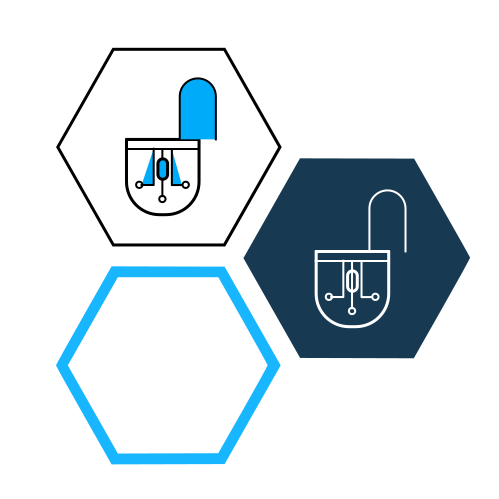
\includegraphics[width=60mm,scale=0.5]{cfg-icons/CFG_ehrenamtliche_edit.png}
	\labfig{ehrenamtliche}
\end{marginfigure}

Dieser Leitfaden richtet sich an Verwaltungen und ähnliche Einrichtungen, die selbst einen Hackathon organisieren möchten. Er fasst die Erfahrungen von Akteur:innen der Civic-Tech-Community zusammen und gibt Anregungen, was ein Hackathon leisten kann – und was nicht.

Dieses Dokument soll einen ersten Überblick bieten für interessierte Kommunen. Für konkrete Tipps und Hinweise, wie ein Hackathon durchgeführt werden kann, verweisen wir an dieser Stelle auf das Handbuch von Jugend hackt \footnote{https://handbuch.jugendhackt.de/}. Auch hier ist noch ein Wettbewerb beschrieben, der seit 2017 nicht mehr stattfindet und mehr Austausch unter den Jugendlichen ermöglicht. Stattdessen gibt es jetzt eine öffentliche Abschlusspräsentation ohne Bewertung.

Unser Ziel ist es, ein ähnliches Handbuch für Verwaltungen zu verfassen, sobald das im Rahmen unseres ehrenamtlichen Engagements zeitlich möglich ist.

\newpage

\chapter{Was ist ein Hackathon?}
\labsec{does}

Bei einem Hackathon kommen verschiedene Menschen für einen bestimmten Zeitraum – gegebenenfalls virtuell – zusammen, um sich intensiv mit einem Themenfeld auseinanderzusetzen. Das Format kommt aus der Softwareentwicklungsszene und im Kern geht es oft darum, sich in einem beschränkten Zeitraum (meist ein Wochenende) einem bestimmten Problem zu widmen.

Im ursprünglichen Sinn kann es beispielsweise darum gehen, sich auf vielfältige Weise mit einer neuen Programmiersprache oder einer bestimmten Technologie zu beschäftigen. Genauso kann es aber möglich sein, Ideen zu einem bestimmten Themen- oder Problemfeld zu durchdenken und im gesetzten Zeitrahmen einen – meist technischen – Lösungsvorschlag für ein Problem als Konzeptprototypen zu finden und vorstellbar zu machen.

% \marginnote[2mm]{The audacious users might feel tempted to edit some of 	these packages. I'd be immensely happy if they sent me examples of what 	they have been able to do!}

\section*{Mehr als nur ein Prototyp}

Tatsächlich hat sich in der Praxis allerdings herausgestellt, dass positive Ergebnisse eines solchen Formats häufig nicht unbedingt in der Entwicklung eines technischen Prototypen liegen, sondern viel weitreichendere Fortschritte erzielen können.

Die Empfehlungen hier zielen auf kommunale und andere öffentliche Institutionen ab. Hackathons im wirtschaftlichen Zusammenhang haben in der Regel etwas andere Schwerpunkte.

\begin{marginfigure}[-10.5cm]
	\includegraphics[width=60mm,scale=0.5]{cfg-icons/CFG_netzwerk_edit.png}
	\labfig{netzwerk}
\end{marginfigure}

Hackathons eignen sich hervorragend, um

\begin{itemize}
	\item \textbf{persönliche Beziehungen aufzubauen}, \newline beispielsweise von der Verwaltung zur lokalen Gruppe von Aktiven im Civic-Tech-Bereich – und den verschiedenen Gruppen untereinander. 
	\vspace{0.5cm}
	\item \textbf{interessierte Menschen zusammenzubringen} \newline und so nicht nur persönliche Vernetzung vor Ort, sondern auch Wissensaustausch zu ermöglichen. Hier ist insbesondere die Vernetzung von Verwaltungsbeschäftigten mit den Teilnehmenden zu nennen, aber auch untereinander. Nicht selten treffen in der Vorbereitung und Durchführung solch einer Veranstaltung erstmals Personen aufeinander, die jeweils gegenseitig einen Nutzen aus der freien Verfügbarkeit von Daten der jeweils anderen Partei ziehen könnten.
	\vspace{0.5cm}
	\item \textbf{Bestehende Ansatzpunkte und Systeme identifizieren}, \newline die lokal in der Verwaltung umgesetzt werden können. Häufig muss hierfür nichts Neues erfunden oder gebaut werden, sondern es geht um die Anpassung und den Betrieb bereits bestehender und gut funktionierender Systeme. Während der Corona-Pandemie haben beispielsweise die Berliner Bäder begonnen, ihre Schwimmzeiten über das Open-Source-Ti\-cket\-verkauf\-ssystem \textit{pretix} zu vergeben. Dieses System hatte sich Jahre zuvor insbesondere im Veranstaltungsbereich bewährt.
	\vspace{0.5cm}
	\item \textbf{Schwachstellen der kommunalen IT-Struktur erkennen}, \newline an denen die Umsetzung solcher Ideen bislang scheitert. Beim beschriebenen \textit{pretix}-System beispielsweise: Was hindert die lokale Verwaltung bislang, dieses System für eigene Zwecke zu installieren und zu betreiben? Ansatzpunkt kann aber auch sein, niederschwellig zugängliche Infrastruktur zu identifizieren – analog z.B. zu Bibliotheken – die es der Zivilgesellschaft ermöglichen würde, die vorgestellten Ideen auch außerhalb eines solchen Formats das ganze Jahr über voranzutreiben.
\end{itemize}


\section*{Ein Format – viele Möglichkeiten}

In den meisten Fällen dauert ein Hackathon zwei oder drei Tage. In dieser Zeit wird häufig in festen Teams gearbeitet – mindestens genauso wichtig ist allerdings die Zeit am Buffet, in kurzen Input-Präsentationen zwischendurch oder in Workshops, bei den die Teilnehmenden neue Techniken erproben oder Fertigkeiten erlernen können.

\begin{marginfigure}[-0.5cm]
	\includegraphics[width=60mm,scale=0.5]{cfg-icons/CFG_projekte_edit.png}
	\labfig{projekte}
\end{marginfigure}

Das Format kann aber auch über längere Zeiträume betrieben werden. Dies kann in bestimmten Fällen vorteilhaft sein, beispielsweise bei internationaler Zusammenarbeit, oder wenn eine Recherche- oder Einarbeitungsphase sinnvoll ist. Der Kulturhackathon \textit{Coding da Vinci} ist beispielsweise in zwei Veranstaltungsblöcke mit einer dazwischen liegenden, mehrere Wochen dauernden Umsetzungsphase aufgeteilt.

Genauso gibt es Hackathons, die nur einen Tag dauern und wo sich überwiegend Menschen treffen, die sich bereits kennen, um gemeinsam fokussiert an einem Ziel zu arbeiten – beispielsweise an einem Leitfaden wie diesem.

Während vor dem Ausbruch der Corona-Pandemie die meisten Hackathons vor Ort stattfanden, übertrugen immer mehr Organisator*innen ihre Konzepte in Online-Veranstaltungen. Auch Kombinationen aus beiden Formaten wurden erprobt.

Gleichzeitig haben immer mehr Branchen das Hackathon-Format für sich entdeckt.




\begin{kaobox}
	Grundsätzlich gilt: Ein Hackathon ist immer, was man daraus macht. \textit{\textbf{Den}} Hackathon gibt es nicht.
\end{kaobox}

Allerdings gibt es viele falsche Vorstellungen davon, welche Ergebnisse ein Hackathon liefern kann und sollte. Mit den gängigsten Vorurteilen räumt der nächste Abschnitt auf.

\vspace{8cm}
\begin{figure*}[h!]
	\includegraphics[width=16cm,scale=0.5]{cfg-icons/CFG_code_wide.png}
\end{figure*}

\chapter{Was ein Hackathon nicht leisten kann}

Bei der Bewerbung von Hackathons wird häufig das Ziel propagiert, Prototypen oder noch besser fertige Produkte und lauffähige Softwaresysteme zu erstellen. Die Praxis zeigt jedoch: Für viele der vorgestellten Ideen gibt es bereits vorhandene Ansätze oder gar funktionierende Systeme – teilweise sogar in besseren Versionen, weil sie bereits seit längerem entwickelt werden.

In der Kürze der Zeit ist es auch für eine ausgebildete Fachjury nur schwer möglich, die Qualität und vor allem die Wirksamkeit der präsentierten „Produkte“ angemessen abzuschätzen. Insbesondere wenn ein Preisgeld ausgelobt wird, können Teilnehmende motiviert sein, mehr an der abschließenden Präsentation für eine gute Jurybewertung zu arbeiten, statt inhaltlich aktiv zu werden. So können am Ende nicht nur die Teilnehmenden frustriert sein, sondern auch die Organisator:innen, wenn sie unter Zeitdruck Projekte bewerten müssen und erst im Nachhinein feststellen, dass sie eine bessere Wahl hätten treffen können.

\section*{Wettbewerb als Innovationshemmnis}

Außerdem motiviert ein Wettbewerbs-Charakter dazu, dass die Teilnehmenden in künstlich abgegrenzten Teams gegen- statt miteinander arbeiten.

Manchmal bringen Teilnehmende bereits vorbereitete eigene Lösungen oder von ihnen kommerziell vertriebene Produkte zur Veranstaltung, um dafür oder für andere eigene Inhalte Werbung zu machen. Das ist nicht immer im Sinne der ausrichtenden Institution und führt zumindest in einer Wettbewerb-Konstellation durch die geleistete Vorarbeit zu Verzerrungen.

An welcher Stelle ein Wettbewerb sinnvoll wäre, muss natürlich im Einzelfall enschieden werden. Auch wenn Konkurrenz bekanntlich „das Geschäft belebt“, können darunter wertvolle Kollaboration und der Beziehungsaufbau während des Hackathons, aber auch besonders die Offenheit und die Weiterverwendbarkeit der Ergebnisse leiden.


\begin{marginfigure}[-16.5cm]
	\includegraphics[width=60mm,scale=0.5]{cfg-icons/CFG_labs_edit.png}
\end{marginfigure}


\section*{Lücken finden und schließen}

Geht es also darum, ein ganz konkretes Problem zu lösen, sollten eine gründliche Recherche betrieben und mögliche bereits existierende Lösungsansätze auf anderen Wegen gesucht werden. Bei einem Hackathon können allerdings genausogut neue Impulse entstehen, oder eine Vorstellung, wo man nach weiteren Lösungen suchen könnte. Die Erwartung der fertig konzeptionierten, weltbewegenden neuen Idee wird jedenfalls sehr selten erfüllt.

\begin{kaobox}
	Die größten Probleme lassen sich nicht durch Prototypen lösen. Prototypen können aber helfen, anschaulich zu machen, wie man von einer Erkenntnis zur Umsetzung kommt.
\end{kaobox}

Denn häufig liegt das Problem gar nicht in fehlenden Lösungen, sondern in der fehlenden Umsetzung durch die öffentliche Hand selbst – etwa, weil es an IT-Infrastruktur wie Administrator:innen, Servern oder Schnittstellen mangelt oder die nötige Datenbasis nicht vorhanden ist.

Deshalb kann es sinnvoll sein, statt einem reinen Hackathon ein Barcamp zu veranstalten. Dort muss dann nicht zwangsläufig ein Prototyp entwickelt werden, sondern Vernetzung und Austausch stehen im Vordergrund. Auch hierbei bringen die Teilnehmenden Themen und Ideen ein und können Zeitslots gestalten, in denen sie ihr eigenes Wissen weitergeben oder zur Diskussion einladen.

\begin{marginfigure}[-6.5cm]
	\includegraphics[width=60mm,scale=0.5]{cfg-icons/CFG_code_for_climate_edit.png}
	\labfig{codeforclimate}
\end{marginfigure}


\section*{Technische Lösungen für soziale Probleme}

Viele Hackathons gehen davon aus, dass am Ende ein Prototyp für ein technisches Produkt steht. Vielfach übersehen wird dabei jedoch, wie sich dieses Produkt in ein komplexes soziales System einfügt und welche unerwarteten und unerwünschten Seiteneffekte damit einhergehen können.

Ganz plakativ gesagt: Keine App wird Hunger beenden, Wohnungslosigkeit lösen, Rassismus beenden oder die Verkehrswende herbeiführen. Im Gegenteil kann die Annahme, dass komplexe soziale Probleme einfach durch technische Produkte gelöst werden können, zu weiteren Problemen führen.

Die Teilnehmenden eines Hackathons sind häufig mehrheitlich mehrfach priviligiert. Sie sind in der Regel vorwiegend weiß und männlich, haben guten Zugang zu Bildung, finanziellen Mitteln und damit auch zu Technologie. Wer ein Wochenende bei einem Hackathon verbringen kann, muss nicht alleine ein Kind oder Angehörige pflegen, kann sich gegebenenfalls Reise und Unterkunft leisten und ist nicht darauf angewiesen, während des Veranstaltungszeitraums Lohnarbeit zu leisten. 

Lösungsvorschläge werden dementsprechend häufig aus Sicht dieser Gruppe konzipiert und formuliert. Seiteneffekte auf marginalisierte Gruppen oder auch spezifische Probleme marginalisierter Gruppen finden dabei häufig keinerlei Beachtung. Ein so entwickeltes Werkzeug kann somit bestehende Klüfte zwischen gesellschaftlichen Gruppen noch weiter verschärfen.

\begin{kaobox}
	In der Civic-Tech-Entwicklung wird als Beispiel hier die Anwendung StreetBump genannt. Ziel der Smartphone-App war es, durch den eingebauten Beschleunigungssensor während der Autofahrt Schlaglöcher in Straßen zu erkennen und diese dem Bauhof zur baldigen Ausbesserung zu melden. 
	
	Kritiker:innen merkten an, dass somit Schlaglöcher vor allem dort gemeldet wurden, wo die Bewohner:innen sowohl aktuelle Smartphones besaßen als auch mit einem eigenen PKW fuhren. Im Zweifel wurden so die bestehenden Kapazitäten zugunsten dieser Quartiere mit ohnehin privilegierten Bewohner:innen priorisiert.
	
	Typische weitere Beispiele aus dem Alltag sind automatische Seifen- oder Desinfektionsmittelspender, die nur helle Haut erkennen; Bilderkennungsalgorithmen, die bei nicht-weißen Gesichtern versagen; Eingabeverifizierungssysteme in Formularmasken, die nur das europäische Vor- und Nachnamenssystem verstehen. Dabei ist die Reihenfolge Vor- und Nachname nicht universell, und auch „Wu“ kann ein vollständiger Nachname sein \footnote{Siehe auch folgender Artikel: \url{https://www.kalzumeus.com/2010/06/17/falsehoods-programmers-believe-about-names/}}.
\end{kaobox}


\vspace{0cm}
\begin{figure*}[h!]
	\includegraphics[width=16cm,scale=0.5]{cfg-icons/CFG_open_government_wide.png}
\end{figure*}

% \setchapterimage[6cm]{donut.jpg}
% \setcounter{margintocdepth}{1}
% \setchapterpreamble[u]{\margintoc}
\chapter{Der Hackathon als erster Schritt}

Ein Hackathon als einzelne Veranstaltung wird nur höchst selten konkrete Probleme mit einem technischen Produkt lösen können. Wertvoll wird die Veranstaltung vor allem auf einer anderen Ebene: Wenn sich Menschen aus unterschiedlichen Kontexten und mit unterschiedlichen Perspektiven zusammenfinden, dann findet auch viel informeller Wissensaustausch statt.

\begin{kaobox}
	Welche Erfahrungen hat eine Entwicklerin in einem bestimmten Datenbank-Projekt bereits gemacht und welche Fehler könnte man vermeiden? Wer hat schon einmal eine ähnliche Lösung in einem anderen Kontext gesehen? Wer kennt jemanden, der in einem bestimmten Bereich besondere Expertise hat? Das sind Fragen, die häufig gar nicht vorher formuliert werden können, sondern sich in Gesprächen ergeben.
\end{kaobox}

Damit tauchen auch häufig neue Fragestellungen auf, Annahmen werden plötzlich noch einmal hinterfragt und es werden Schwachstellen in bestehenden Infrastrukturen sichtbar. Beispielsweise benötigt eine App Daten, die zwar in internen Systemen vorhanden, aber nicht frei verfügbar sind. Dieses Dilemma kann in den seltensten Fällen direkt auf dem Hackathon gelöst werden – hier müssen die Mitarbeitenden die Veranstaltung dann entsprechend nachbereiten und für zukünftige Projekte die Daten zugänglich machen.

\begin{marginfigure}[-5.5cm]
	\includegraphics[width=60mm,scale=0.5]{cfg-icons/CFG_open_data_edit.png}
\end{marginfigure}


Genauso bleibt im eng gesteckten Rahmen eines Hackathons häufig offen, wer eine bereits bestehende, funktionierende Lösung betreiben kann.

\section*{Der Beginn einer langen Reise}

Ein Hackathon ist also weniger eine Produkt-Fabrik als vielmehr ein wirkmächtiger Ausgangspunkt für einen strukturellen Wandel – allerdings natürlich nur, wenn die Organisator:innen für diese Möglichkeiten sensibilisiert und darauf vorbereitet sind, die nötigen Veränderungen umzusetzen.

Wer einen Hackathon organisiert, sollte daher von Anfang an ausreichende Kapazitäten in der eigenen Organisation für die Nachbereitung der Erkenntnisse in den Monaten nach der Veranstaltung einplanen. Wie kann der Kontakt zu den Teilnehmenden oder auch anderen interessanten Partner:innen aufrechterhalten und vertieft werden? Welche Kompetenzen und welche Prozesse müssen in der Organisation aufgebaut werden? Wo fehlt es gar derzeit an Personal?

Wenn dies nicht passiert, wird der Großteil des Potenzials der Veranstaltung wirkungslos verpuffen. Ein leider nicht unübliches Muster ist, dass zwar Jahr für Jahr bei wiederkehrenden Veranstaltungen jeweils neue Einzeldatensätze bereitgestellt werden, aber keine der Anregungen für strukturelle Verbesserungen in der Organisation verfangen. Im schlimmsten Fall ist dies eine Offenlegung des Umstands, dass die Verwaltung zu nachhaltigem Wandel über reine Show hinaus nicht in der Lage ist. Bei Folgeveranstaltungen kann das dazu führen, dass die Teilnehmenden ausbleiben, weil sie ihre Bemühungen nicht als sinnhaft erleben und sich schlimmstenfalls nicht gehört oder ernst genommen fühlen.

Gelingt es den Organisator:innen allerdings, die Teilnehmenden für die eigenen Problemstellungen zu begeistern und eine Kommunikation auf Augenhöhe zu ermöglichen, kann ein Hackathon eine gute und bereichernde Möglichkeit sein, um die (digitale) Zivilgesellschaft in langfristige Wandlungsprozesse einzubeziehen.


%\begin{marginfigure}[-5.5cm]
%	\includegraphics[width=35mm,scale=0.5]{cfg-icons/CFG_civic_tech.png}
%\end{marginfigure}

\vspace{6cm}
\begin{figure*}[h!]
	\includegraphics[width=14cm,scale=0.5]{cfg-icons/CFG_civic_tech_wide.png}
\end{figure*}


% \marginnote[2mm]{The audacious users might feel tempted to edit some of these packages. I'd be immensely happy if they sent me examples of what they have been able to do!}

